\footnotesize
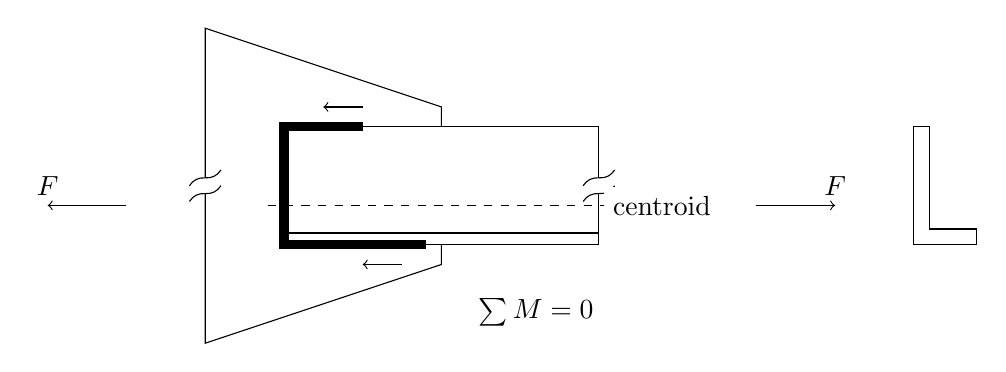
\begin{tikzpicture}[scale=1,ext/.pic={
\path[fill=white](-0.2,0)to[bend left](0,0.1)to[bend right](0.2,0.2)to(0.2,0)to[bend left](0,-0.1)to[bend right](-0.2,-0.2)--cycle;
\draw(-0.2,0)to[bend left](0,0.1)to[bend right](0.2,0.2) (0.2,0)to[bend left](0,-0.1)to[bend right](-0.2,-0.2);
}]
\draw(2,-1)--(2,1)--(-1,2)--(-1,-2)--cycle;
\draw[fill=white](0,-.75)rectangle(4,.75);
\draw(0,-.6)--(4,-.6);
\draw(4,0)pic{ext};
\draw(-1,0)pic{ext};
\draw[dashed](-.2,-.25)--++(5,0)node[fill=white]{centroid};
\draw[line width=1.2mm](1,.75)-|(0,-.75)--++(1.8,0)node[below right=5mm]{$\sum{}M=0$};
\draw[->](-2,-.25)--++(-1,0)node[above]{$F$};
\draw[->](6,-.25)--++(1,0)node[above]{$F$};
\draw[->](1,1)--++(-.5,0);
\draw[->](1.5,-1)--++(-.5,0);
\begin{scope}[xshift=8cm]
\draw(0,-.75)|-(.2,.75)|-(.8,-.55)|-cycle;
\end{scope}
\end{tikzpicture}